
% viimeinen kappale tarvitsee uudelleen kirjoituksen
% jsx kohta tarpii vähän uudelleen kirjoittamista

\subsubsection{React Yleisesti}






% https://github.com/facebook/react/blob/main/README.md
% https://github.com/facebook/react/blob/f74c5ccf9469d3389ce3a1ee3b54988049e235f7/README.md
% https://www.infoq.com/news/2013/06/facebook-react/
% molemmat siteerattu 27.5.24

%https://opensource.fb.com/projects/react/
% 12.6

% https://react.dev/
% 30.5


%https://www.statista.com/statistics/1124699/worldwide-developer-survey-most-used-frameworks-web/
%yksi käytetyimmistä työkaluista 
% 30.5





React on Metan ylläpitämä avoimeen lähdekoodiin perustuva javascript kirjasto,
joka on suunniteltu reaktiivisien käyttöliittymien kehittämiseen\labcite{react24a}
React kannustaa kehittäjiä rakentamaan sovelluksia uudelleenkäytettävien komponenttien avulla.
Jokainen komponentti sisältää oman rakenteensa, tyylinsä ja käyttäytymisensä, joka tekee niistä helposti siirrettävän ja uudelleenkäytettävän.\labcite{react24a}
Komponenteista voidaan sitten koota monimutkaisia käyttöliittymiä. 
\medskip


Komponentit voidaan kirjoittaa JSX (eng JavaScript XML) syntaksilla, joka mahdollistaa HTML tyylisen kirjoituksen JavaScriptin sekaan.
Tämä tekee React:ista helppo luettavan, ymmärrettävän ja opittavan,
joka on auttanut nostamaan Reactin suosiota yhteen maailman käytetyimmistä käyttöliittymä työkaluista.\labcite{statista23a}
\medskip









\subsubsection{JSX}





%https://react.dev/learn/writing-markup-with-jsx
%https://facebook.github.io/jsx/ 

% jsx = js xml
% https://medium.com/@sjarancio/what-is-jsx-e3dda0af3490

%transpilation
% https://www.scholarhat.com/tutorial/react/getting-started-with-jsx
% https://www.typescriptlang.org/docs/handbook/jsx.html

% kaikki viitattu 27.5







JSX on syntaksi jatke JavaScriptille, joka antaa kehittäjän kirjoittaa HTML tyylistä syntaksia JavaScriptin sekaan,
tehden koodista yksinkertaisempaa ja helpompaa ymmärtää\labciteend{Stephen21}
JSX ei ole ECMAscript standardissa, joten selaimet eivät osaa tulkita sitä,
vaan JSX se on suunniteltu transpiloitavaksi johonkin ECMAscript standardia toteuttavalle kielelle\labciteend{Facebook22}
\medskip



% tämä on jotenkin scuffed. se pitäisi kirjoittaa kokonaan eri tavalla%
% en tykkää että tehdään muuttuja. (se on muutenkin const)
%  en kyllä tiedä mikä muu se voisi olla

% muutenkin pitäisi varmaan liimata jsx paremmin tähän paragraafiin


Kuvassa \nextImageCount{} luodaan muuttuja helloWorld, jolle annetaan arvoksi HTML "p"{} elementti, jossa teksti "Hello, World!"{}.
Muuttujien arvot voidaan kirjoittaa HTML tyylisellä JSX syntaksilla, 
joka tekee komponenttien määritelmästä helppoluettavan.
\medskip



\bigskip
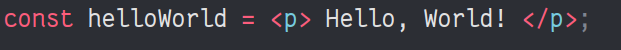
\includegraphics[width=10cm]{src/public/oppar/pure_jsx_example.png}\\
Kuva \getImgCount {}. Esimerki JSX syntaxista
\medskip



% tämäkin on vähän scuffed sillä kuvan alla puhutaan jo seuraavasta kuvasta eikä mainita muuttaa
% en tiedä onko tämä oiikeaa tyyliä
%  voisi mainita uudelleen että selain ei voi suorittaa jsx joten asialle pitää tehdä jotain jos halutaan että toimii
% sitten mainita seuraavasta kuvasta ja jne

Selaimet eivät voi tulkita JSX syntaksia, joten se pitää transpiloida natiiviin JavaScriptiin.
Kuvassa \nextImageCount{} on kuvan \theimgCounter{} helloworld muuttuja, joka on transpiloitu natiiviksi JavaScriptiksi Babel kääntäjää käyttäen. \labcite{babel24}
Tämä antaa selaimille mahdollisuuden suorittaa koodia, joka on alkuperin kirjoitettu JSX syntaksilla.
\medskip


\bigskip
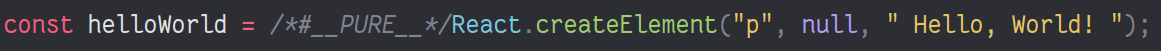
\includegraphics[width=15cm]{src/public/oppar/transpiled_jsx_example.png}\\
Kuva \getImgCount {}. Kuvan \prevImageCount{} JSX transpiloitu JavaScriptiin
\medskip





\subsubsection{Komponentit}




% kolmas kappale pitää korjata 
% kapale ennen kuvaa tarvitsee lisää sanaa


% komponentti joka voi renderöidä toisen komponentin. tämä jatkuu siihen asti että päästään natiiveihin html elementteihin jotka selain osaa tulkita
%https://react.dev/learn/your-first-component



%tarvitsee korjailua

% åitää selittää mikä itse se on. eli 
% elementti joka joka sisältää oman jne jen

Komponentti on oma pieni kokoonpano, joka sisältää sen ulkonäön ja käyttäytymisen.
Komponentit ovat olennainen rakennusosa React sovelluksissa.
Reactissa Komponentit voivat olla tilallisia tai tilattomia.\labcite{react24d} 
\medskip



Tilaton komponentti ei sisällä omaa tilaa. 
Niiden pää tarkoitus on renderöidä käyttöliittymää niille annettujen propertyjen perusteella.
Tilattomat komponentit on helpompi kirjoittaa ja testata verrattuna tilalliseen komponenttiin, 
sillä niissä ei ole sivu efektejä eikä niiden käytäntö tai ulkonäkö vaihdu sisäisen tilan takia.\labcite{Phuoc23}
\medskip


Tilallinen komponentti tarkoittaa komponenttia, 
joka sisältää oman tilan ja on vastuussa sen hallinnoinnista ja päivittämisestä.
Tilalliset komponentit ovat tarkoitettu käyttää, kun käyttöliittymässä tarvitsee säilyttää dataa ajanmyötä 
kuten lomake tietoja.\labcite{Phuoc23}\\
\medskip




%tähän voisi periaatteessa liimata sen preamblen tosta luokkakomponentti kohdasta
% sitten olisi tarpeeksi tekstiä tässä ja se voisi olla vähän tiivimmän näköinen



React tukee kahta tapaa luoda komponentteja. Luokkakomponentti ja funktiokomponentti.\labciteend{react24c}
Molemmilla komponentti tyyleillä voidaan toteuttaa samanlaisia komponentteja, mutta React on kehottaa käyttää funktiokomponentteja tulevaisuudessa. \labcite{react24c}
Kuvassa \nextImageCount {} on esimerkki tilallisesta funktiokomponentista ja
kuvassa \nextnextImageCount {} on sama laskukomponentti kuin kuva \nextImageCount{} mutta kirjoitettu luokkakomponentti tyylillä. 
\medskip


\bigskip
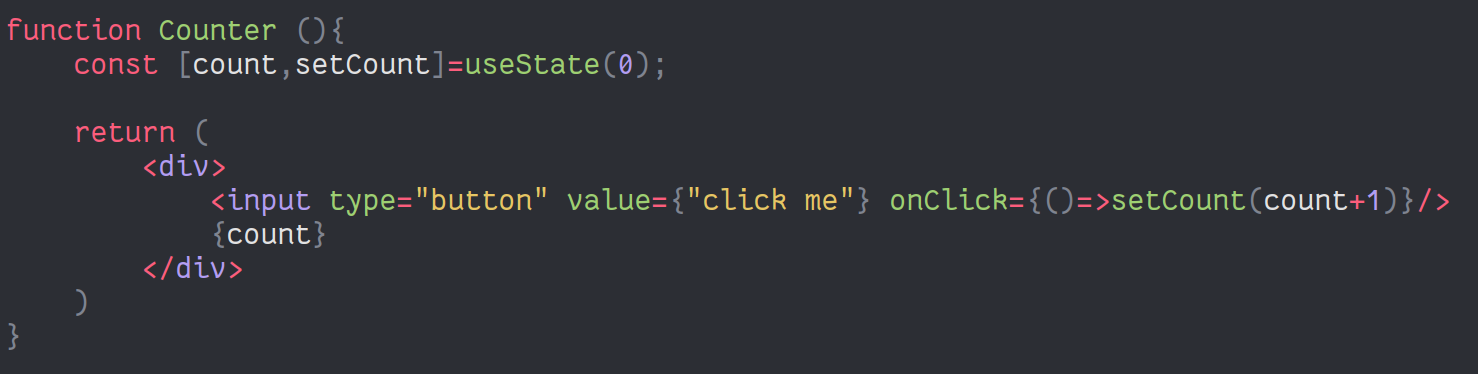
\includegraphics[width=15cm]{src/public/oppar/function_component.png}\\
Kuva \getImgCount{}. kuvakaappaus React komponentista(KORJAA INDENTAATIO)
\medskip

Kuvaassa \theimgCounter{} määritetään funktiokomponentti, jonka nimeksi on annettu laskija, joka seuraa kuinka monta kertaa nappia on painettu.
Funktio palauttaa komponentin ulkonäön, joka on määritetty JSX syntaksilla.
Komponentissa on myös useState "hook"{}, joka kuvastaa komponentin tilan,
tätä käyttäen komponentti pystyy säilyttämään dataa ja päivittämään itsensä, kun sen sisäinen tila muuttuu.
\medskip




\bigskip
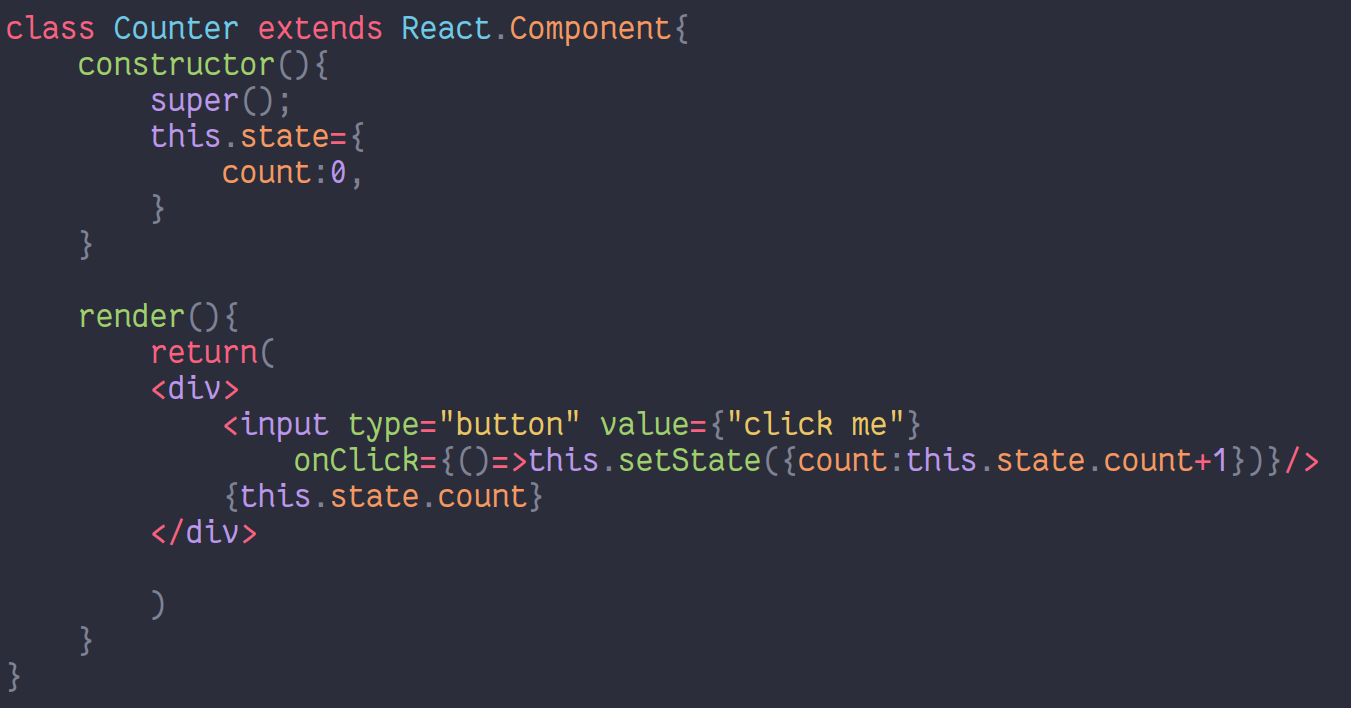
\includegraphics[width=15cm]{src/public/oppar/class_.png}\\
Kuva \getImgCount{}. kuvakaappaus React luokkakomponentista(POISTA CURSOR KUVASTA)
\medskip



Luokkakomponentissa komponentin tilaa säilytetään this.state ominaisuudessa, ja sitä voi muuttaa tai päivittää käyttämällä this.setState funktiolla. 
Funktio uudelleen renderöi osat komponentista jotka, ovat riippuvaisia kyseisestä tilasta.\labciteend{react24c}
\medskip


Funktiokomponentissa tila hallinnoidaan "React hookeilla"{}. 
"Hookit"{} antavat funktiokomponenteille mahdollisuuden käyttää Reactin ominaisuuksia, 
jotka luokkakomponentit saavat, kun ne jatkavat Reactin "Component"{} luokkaa.\labcite{react24b}
Kuvan \prevImageCount{} ja \theimgCounter{} komponentit ovat tehty React 18.3.1 versiolla.
\medskip



\subsubsection{DOM ja VDOM}



%psychotic
% dom ei ole pakko olla puu formaatti se pitää mainita
% eli kirjoita tämä koko shid uudellee
%DOM (eng Document object model) on puu-struktuurinen representaatio HTML dokumentista.
%Tätä struktuuria käytetään rajapintana JavaScriptin ja HTML:län välillä. 
%Struktuurissa jokainen solmu on objekti, joka esittää osaa dokumentista. 
%Soulmuissa voi olla yksi tai useampi objekti ja nämä objektit voivat osoittaa muihin solmuihin.\labcite{w3org}


DOM (eng Document object model) on rajapinta HTML ja XML dokumenteille. 
se määrittää loogisen struktuurin dokumenteista ja määrittää tavan miten dokumenttia hallinnoidaan.
Dom mallissa dokumentit esitetään puu struktuurilla, mutta DOM ei määritä että dokumentit toteutetaan puu struktuurilla.
Struktuurissa jokainen solmu on objekti, joka esittää osaa dokumentista. 
Soulmuissa voi olla yksi tai useampi objekti ja nämä objektit voivat osoittaa muihin solmuihin.\labcite{w3org}
\bigskip



    
%pitää viitata jotenkin
\begin{tcolorbox}
\begin{lstlisting}[language=html]
<TABLE>
    <ROWS> 
      <TR> 
          <TD>Shady Grove</TD>
          <TD>Aeolian</TD> 
      </TR> 
      <TR>
          <TD>Over the River, Charlie</TD>
          <TD>Dorian</TD> 
      </TR> 
    </ROWS>
</TABLE>
\end{lstlisting}
\end{tcolorbox}
%this is not propper need to cite this propperly
% idk how
Koodi 1. html koodista\labimgcite{w3org}
\medskip


Esimerkki HTML koodissa luomme pöydän, jossa tehdään kaksi riviä ROWS elementin alle. 
Joka riviin tulee kaksi "table data"{} elementtiä, jotka sisältävät datan tekstinä.
Kuvassa \nextImageCount {} koodi 1 on muotoiltu DOM puuhun.
%something here???


\bigskip
%kuva html domista
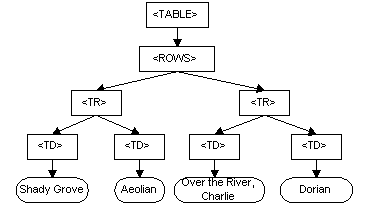
\includegraphics{./src/public/oppar/dom.png}\\
Kuva \getImgCount {}. DOM puu esimerkki HTML koodista \labimgcite{w3org}
\medskip


% en tiedä puuttuuko jotain kappaleesta

DOM toimii rajapintana HTML ja XML dokumentteihin.\labcite{w3org}
Päivityksien tekeminen DOM rajapintaa käyttäen on helppoa, mutta se tulee suorituskyvyn hinnalla.
Elementin päivittäminen DOM:issa päivittää kyseisen elementin kaikki lapsielementit. 
Tästä päivityksestä voi tulla hyvin kallis, jos elementtejä on paljon.\labcite{refine23}
\bigskip



% bharathkumar23 on ehkä huono source joten kokeile kokonaan refine jos on fine
% en tiedä miks ei oo off


Käyttöliittymä päivityksien nopeuttamiseksi React on ottanut käyttöön VDOM:in (eng virtual DOM).
VDOM on virtuaalinen esitys DOM:ista, jonka React pitää muistissaan koko suorituksen ajan\labciteend{refine23}
Elementtien päivittely yksi kerrallaan DOM:iin jokaisen päivityksen ohessa olisi hidasta,
joten React tekee ensiksi kaikki päivitykset VDOM:iin, jonka jälkeen päivityksen DOM:iin voidaan tehdä samanaikaisesti.
%
%
\medskip

Kun React tekee muutoksia VDOM:iin se luo uuden VDOM puun, jonka jälkeen
React määrittää mitkä osat käyttöliittymästä ovat muuttuneet erottelu prosessilla (eng diffing).
Erottelu prosessin ansiosta React tietää mikä on pienin määrä muutoksia mitä pitää tehdä DOM:iin, 
että käyttöliittymä pysyisi ajan tasalla.\labcite{refine23}
\medskip



